\documentclass[10pt,twocolumn,letterpaper]{article}

\usepackage{wacv}
\usepackage{times}
\usepackage{epsfig}
\usepackage{graphicx}
\usepackage{amsmath}
\usepackage{amssymb}

% Include other packages here, before hyperref.

% If you comment hyperref and then uncomment it, you should delete
% egpaper.aux before re-running latex.  (Or just hit 'q' on the first latex
% run, let it finish, and you should be clear).
%\usepackage[pagebackref=true,breaklinks=true,letterpaper=true,colorlinks,bookmarks=false]{hyperref}

%\wacvfinalcopy % *** Uncomment this line for the final submission

\def\wacvPaperID{****} % *** Enter the wacv Paper ID here
\def\httilde{\mbox{\tt\raisebox{-.5ex}{\symbol{126}}}}

% Pages are numbered in submission mode, and unnumbered in camera-ready
\ifwacvfinal\pagestyle{empty}\fi
\setcounter{page}{1}
\begin{document}

%%%%%%%%% TITLE
\title{FlowChroma - A Deep Recurrent Neural Network for Video Colorization}

% Authors at the same institution
%\author{First Author \hspace{2cm} Second Author \\
%Institution1\\
%{\tt\small firstauthor@i1.org}
%}
% Authors at different institutions
%\author{First Author \\
%Institution1\\
%{\tt\small firstauthor@i1.org}
%\and
%Second Author \\
%Institution2\\
%{\tt\small secondauthor@i2.org}
%}

\maketitle
\ifwacvfinal\thispagestyle{empty}\fi
%%%%%%%%% ABSTRACT
\begin{abstract}
   We develop an automated video colorization framework that minimizes the flickering of colors across frames. If we apply image colorization techniques to successive frames of a video, they treat each frame as a separate colorization task. Thus, they do not maintain the colors of a scene consistently across subsequent frames.

The proposed solution includes a novel deep recurrent encoder-decoder architecture which is capable of maintaining contextual information between consecutive frames of a video. We use a high-level semantic feature extractor to automatically identify the context of a scenario, with a custom fusion layer that combines the spatial and temporal features of a frame sequence. We demonstrate experimental results, qualitatively showing that recurrent neural networks can be successfully used to improve color consistency in video colorization.
\end{abstract}

%%%%%%%%% BODY TEXT
\section{Introduction}
Colorizing a grayscale image to achieve a natural look has been a much-explored research problem in the recent years, especially with the rise of deep learning-based approaches for image processing. A primary goal has been to produce diverse colorizations, while also providing plausible colorizations that apply correct colors to identified objects. Desaturating an image is a surjective operation, but it is not injective. Hence, there are multiple possible colors to choose from when considering a pixel in a grayscale image --– it is a one-to-many mapping.

Compared to the image colorization problem, colorizing black and white videos has largely been left behind. This problem has abundant training data, as one could easily desaturate a video and test the colorization against the original video. Video colorization could be used as a video preprocessing technique, such as to enhance CCTV footage, and to restore old movies and documentaries. One could argue that video colorization could be taken as a direct extension of image colorization, where successive application of frame colorization would produce a colorized video. But obviously, there is no guarantee that the selected image colorization technique would color successive frames consistently, known as temporal coherence, since it would consider each frame as a separate task, ignoring the contextual connections between frames.  This would result in flickering colors, reducing the usefulness of such results.

\raggedbottom
The other prime obstacle has been the high computational costs in colorizing videos \cite{Levin:2004:CUO:1015706.1015780,6575125} --– it adds another dimension across time on top of the already computationally intensive image colorization.

Another problem is that most of the current image colorization techniques require some sort of human intervention to produce good results, such as user scribbles that guide the colorization process \cite{Levin:2004:CUO:1015706.1015780, DBLP:journals/corr/ZhangZIGLYE17}. While this is feasible for a few images, it certainly does not scale up for videos with thousands of consecutive frames, as commercial videos run at 24 or higher frames per second. Thus, efficiently colorizing a video with resource constraints and minimal supervision poses an interesting research problem.

There's a plethora of early video content shot in black and white that was enjoyed by older generations and remembered fondly. Such classical content is mostly forgotten and the later generations prefer colored content. Colorizing existing content is much cheaper than reproducing them entirely in color today. The financial incentives for colorizing classical content have never been higher, as it opens up new content for the millennials and later while giving a chance for Generation X and earlier to reminisce.

Our research contributions are as follows; (1) We propose a new fully automated video colorization framework focusing on improved temporal and contextual coherence between frames and scene changes. (2) We use a Recurrent Neural Network (RNN) based architecture for the first time in the colorization domain, to maintain contextual information across frames for consistent coloring. (3) We study the effects of using RNNs on the colorization of videos.

%-------------------------------------------------------------------------
\section{Related Work}

Most of the previous work in the colorization domain has been done for image colorization, leaving video colorization largely unexplored. Lots of algorithms have been developed to solve the image colorization problem and they fall into two major categories: parametric methods \cite{DBLP:journals/corr/abs-1712-03400, DBLP:journals/corr/ChengYS16, 7410429, Iizuka:2016:LCJ:2897824.2925974, DBLP:journals/corr/LarssonMS16, DBLP:journals/corr/ZhangIE16, DBLP:journals/corr/ZhangZIGLYE17} and non-parametric methods \cite{10.1007/978-3-540-88690-7_10, Chia:2011:SCI:2070781.2024190, Gupta:2012:ICU:2393347.2393402, Huang:2005:AED:1101149.1101223, Irony:2005:CE:2383654.2383683, Levin:2004:CUO:1015706.1015780, Luan:2007:NIC:2383847.2383887, Morimoto:2009:ACG:1599301.1599333, qu-2006-manga, 1467343, Welsh:2002:TCG:566654.566576, 1621234}. Parametric methods learn predictive functions from large datasets of color images. Once the predictive function's parameters are learned with an appropriate optimization objective, it is ready to predict colors of grayscale images in a fully automatic manner. On the other hand, non-parametric methods need some level of human intervention when colorizing images.  

There are mainly two non-parametric methods that are being discussed in the literature: scribble-based and transfer-based. Scribble-based colorization schemas \cite{Huang:2005:AED:1101149.1101223, Levin:2004:CUO:1015706.1015780, Luan:2007:NIC:2383847.2383887, qu-2006-manga, 1621234} require manually chosen color scribbles on the target grayscale image. There are a few instances where the scribble-based colorization methods are extended to video colorization as well. 

Transfer-based colorization schemas \cite{10.1007/978-3-540-88690-7_10, Chia:2011:SCI:2070781.2024190, Gupta:2012:ICU:2393347.2393402, Irony:2005:CE:2383654.2383683, Morimoto:2009:ACG:1599301.1599333, 1467343, Welsh:2002:TCG:566654.566576} require the user to select semantically similar colorful reference images to match similar segments of the target grayscale image with those of colorful reference images. 

Applying non-parametric methods on both image colorization and video colorization has a number of drawbacks, the most prominent among which is the inability to fully automate the colorization process. In color transferring approaches, there is a manual intervention in searching for colorful reference images. Scribble-based colorization may require tens of well-placed scribbles plus a carefully chosen rich pallet of colors in order to achieve convincing natural results for a complex image.  

Both scribble-based and transfer-based video colorization schemas can only be automated within a frame sequence without a scene change; i.e. at each scene change, if the process is scribble-based, the user will have to introduce a new set of scribbles. If it is transfer-based, a new selection of swatches with or without a new reference image will be required. 

The most prominent advantage of parametric colorization schemas is their ability to fully automate the colorization process. Deshpande et al. \cite{7410429} proposed a parametric image colorization schema which formulates the colorization problem as a quadratic objective function and trained it using the LEARCH framework \cite{Ratliff2009}. With the unparalleled successes of deep neural networks, solutions that utilize DNNs have been proposed as parametric image colorization schemas. Cheng et al. \cite{DBLP:journals/corr/ChengYS16} proposed an image colorization schema which leverages a three-layer fully connected neural network that was trained by the inputs of a set of image descriptors: luminance, DAISY features \cite{4587673} and semantic features.  More recently,  many authors have employed CNNs in their colorization schemas rather than conventional DNNs. Zhang et. al. \cite{DBLP:journals/corr/ZhangIE16} proposed a CNN-based colorization schema which predicts a probability distribution of possible colors for each pixel in order to address the typical ambiguous and multimodal nature of image colorization \cite{10.1007/978-3-540-88690-7_10}.

More recently, Zhang et al. \cite{DBLP:journals/corr/ZhangZIGLYE17} introduced a CNN based color recommender system that propagates user-provided scribbles while satisfying high level color preferences of the user. Larsson et al. \cite{DBLP:journals/corr/LarssonMS16} trained an end-to-end network to predict colors of an image with the hypercolumns \cite{DBLP:journals/corr/HariharanAGM14a} for each pixel generated from a pre-trained VGG-16 network without a classification layer. Iizuka et. al. \cite{Iizuka:2016:LCJ:2897824.2925974} proposed a colorization method that utilizes a CNN based architecture, combining a high-level semantic feature extractor, a mid-level feature network and a colorization network. More recently, inspired by the colorization model of Iizuka et. al., Baldassarre et. al. \cite{DBLP:journals/corr/abs-1712-03400} replaced the high-level semantic feature extractor in the colorization model of Iizuka et. al. with a pre-trained CNN image classifier: Inception-ResNet-v2 \cite{DBLP:journals/corr/SzegedyVISW15}. This transfer learning approach significantly reduces the computational time as well as the need for extreme amounts of data and hardware resources to train the colorization network to yield a quality colorization result.

Most of the fully-automatic, parametric image colorization solutions can be extended to video colorization domain by treating a video merely as a sequence of independent frames. But considering video frames independently causes colors to shift erratically, failing to maintain temporal coherence throughout the frame sequence, causing visual fatigue for viewers. i.e. if a certain object or section in a past frame has some color, then a subsequent, contextually related frame should have the same color for the same object or section. For an example, a wall in one frame may be colored in one shade of yellow and the same wall should maintain that color in subsequent frames, rather than changing to a shade of white. Failing to capture these details drastically reduces the quality of colored videos, because the user can notice color mismatches and flickering between video frames. In this research, we explore the effectiveness of employing RNNs to preserve the temporal coherence in video colorization while mitigating the challenges of computational time, need for extreme amounts of data and hardware resources with a transfer learning application.

\section{Approach}

\begin{figure*}
	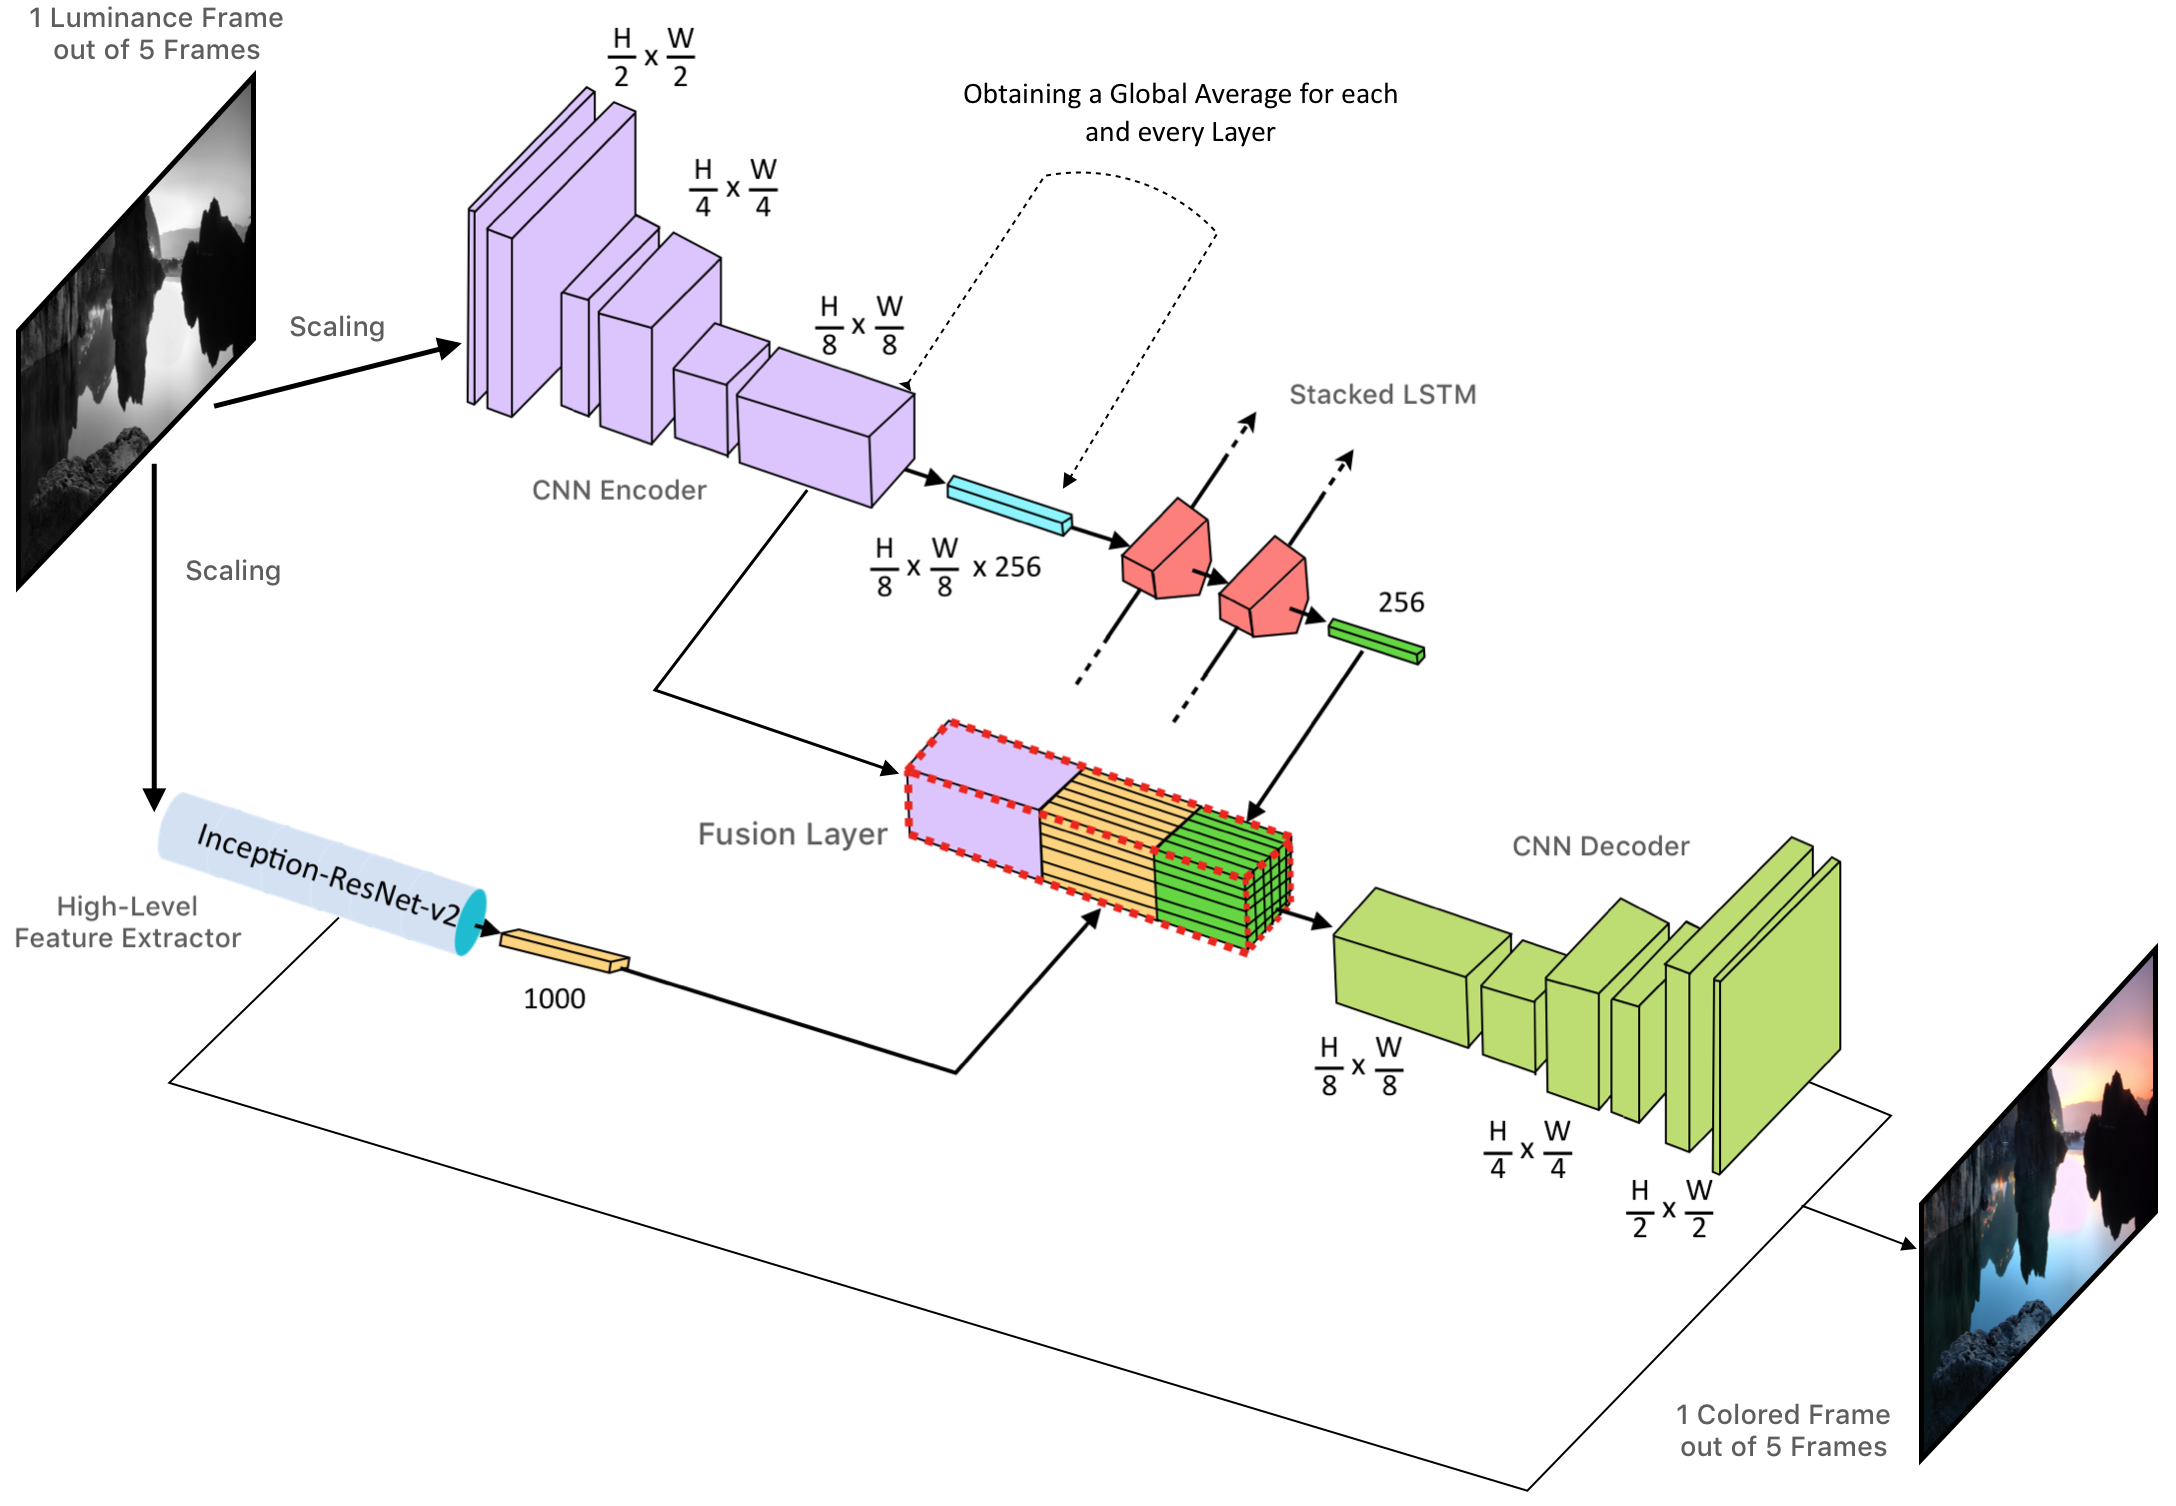
\includegraphics[width=\textwidth]{flowchroma-architecture.png}
\end{figure*}

\begin{figure*}
	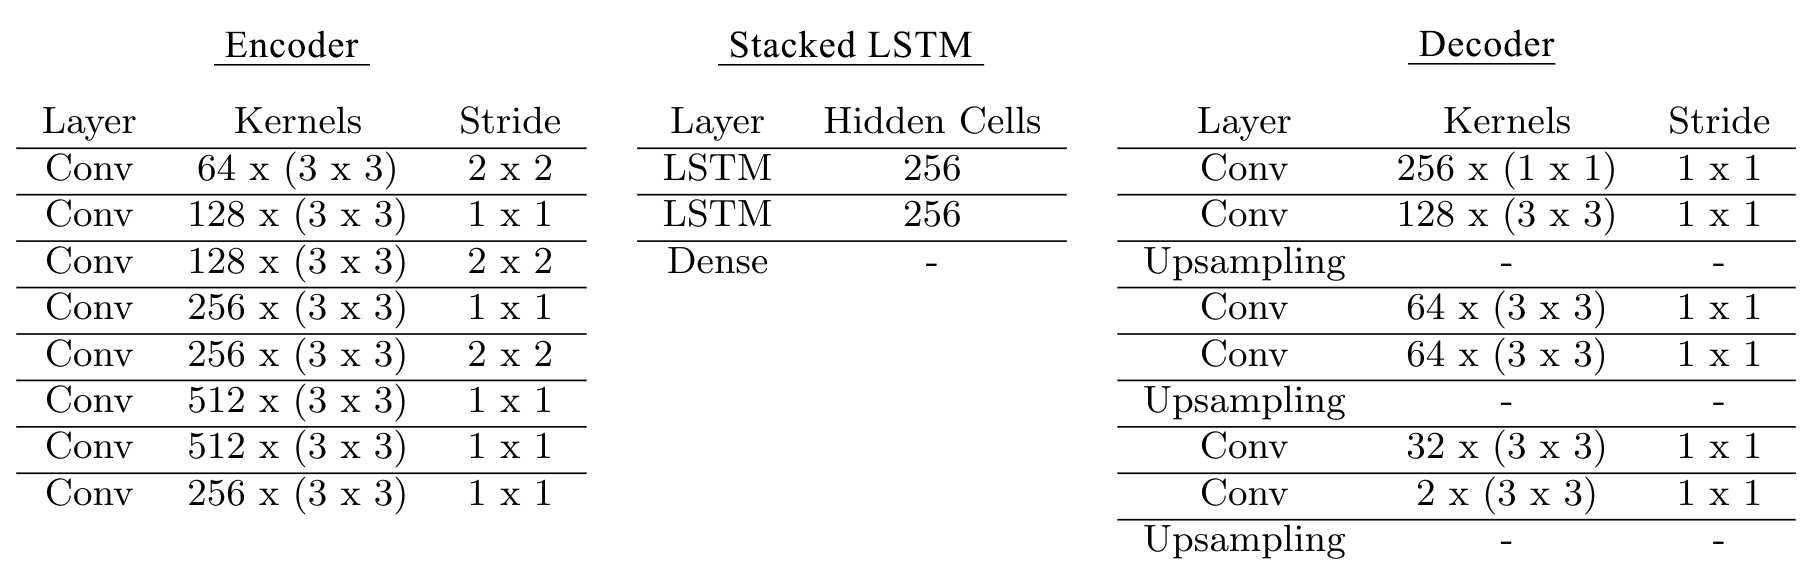
\includegraphics[width=\textwidth]{kernel-stride-table_1.jpg}
    \caption{FlowChroma Architecture: The CNN encoder extracts local features while the Inception network extracts high level semantic information from a frame. The stacked LSTM grasps temporal features from a sequence of frames. The outputs from the CNN encoder, Inception network and the LSTM are then fused together in the fusion layer to provide inputs to the colorization network or the CNN decoder. Note that the CNN encoder, decoder, fusion layer and Inception network are all applied to every temporal slice of the input.}
\end{figure*}

When modeling the video colorization problem as a learnable function, we have chosen the CIE La*b* color space to represent video frames. According to Ruderman et al.\cite{Ruderman98statisticsof}, La*b* color space was developed to minimize correlation between the three coordinate axes of the color space. La*b* color space provides three decorrelated, principal channels corresponding to an achromatic luminance channel L and two chromatic channels as a* and b*. 
If we have a grayscale frame, that means we already have the luminance layer of that particular frame, the next step is finding a plausible a*, b* combination and fusing them together to come up with a final colored frame, given that there is temporal coherence when predicting a* and b* combinations. Therefore, the main assumption here is that for every luminance component of video frames \begin{equation} X\textsubscript{t}^L\in R\textsuperscript{H$\times$W$\times$1} \end{equation} there exists a function F such that \begin{equation}F: \{X\textsubscript{t}^L, X\textsubscript{t-1}^L,..., X\textsubscript{t-(T-1)}^L\} \rightarrow (X\textsubscript{t}\textsuperscript{a$^\ast$}, 
X\textsubscript{t}\textsuperscript{b$^\ast$})\end{equation}  
Here, $X_{t}\textsuperscript{k}$ represents the $k$ layer in $t\textsuperscript{th}$ time frame, H and W the frame height and width respectively, and T represents the total number of time steps.

The chromatic channels a* and b* defines an Euclidean space where the distance to the origin determines the chroma. Change of values in one channel imposes minimal effect on values of the other two, this decorrelation of the three channels allows us to combine the luminance with the predicted chromatic channels, ensuring an image construction with high level of detail but with almost non-existent cross-channel artifacts.

\subsection{Proposed Architecture}

The video sequence colorization process of our model can be divided into five main components; as shown in Figure 1, the CNN encoder, global feature extractor, stacked LSTM, fusion layer and the CNN decoder. We include Inception-ResNet-v2 network as a global feature extractor; this is a transfer learning technique, drawing inspiration from the works of Iizuka et al. and Baldassarre et al. This significantly reduces the computational complexity related to training of the model. We use LSTMs in our network to support video colorization for the first time, taking a novel approach in this domain. 

As shown in Figure 1, The CNN encoder extracts local features while the Inception-ResNet-v2 extracts high level semantic information such as objects and environments from an individual frame. A stacked LSTM is being employed to grasp temporal features of a sequence of frames. The outputs from the CNN encoder, Inception network and the LSTM are then fused together in the fusion layer to provide inputs to the colorization network or the CNN decoder. We assume that the CNN decoder predicts $a*$ and $b*$ layers related to the input luminance frame at the current time step in a spatio-temporal manner.

%-------------------------------------------------------------------------
\subsection{Grasping Local Features of each Individual Frame}
In order to grasp local features of the frame sequence at each time step, we apply a CNN encoder to every temporal slice of the input, it processes a $t\times H\times W$ gray-scale frame sequence and outputs a sequence of $t\times H/8\times W/8\times 256$ feature encodings.

\subsection{Grasping Global Features of each Individual Frame}
Global features such as objects and environments are helpful for the CNN decoder to provide an appropriate colorization process. The high-level feature extractor is a pre-trained Inception-Resnet-v2 model without the last SoftMax layer. When training Flowchroma, we keep Inception’s weights static. At each time step, we scale the input luminance frame to $299\times 299$, and then stack itself to obtain a three channel frame in order to satisfy Inception’s input dimensionality requirements, then we feed the resultant frame to Inception and obtain the its logits output or the output before the softmax layer. When combined the results at each time step we get an final embedding of $t\times 1000$ for the entire sequence.


\subsection{Grasping Temporal Features of a Frame Sequence}
In order to grasp temporal features of the frame sequence, we use a 2-layer stacked LSTM model. The CNN encoder provides a local feature encoding of  $t\times H/8\times W/8\times 256$. By employing global average pooling operation on that encoding at each time step, we obtain an embedding of $t\times 256$, which can be used as inputs to the stacked LSTM. Stacked LSTM has two LSTM layers, each having 256 hidden states, thus giving us an output with the dimensions of $t\times 256$. This output improves temporal coherence of the video colorization predictions.

\subsection{Fusing Local and Global Spatial Features with Temporal Features}
Fusing local and global level spatial features with temporal features will be done by a specially crafted fusion layer, first introduced by Iizuka et al. Similar to CNN encoder, we apply the fusion layer to every temporal slice of the input. The fusion layer takes the output embeddings from Inception and stacked LSTM to replicate it $H/8\times W/8$ times and then concatenates them with the output provided by the CNN encoder. The fusion mechanism is more comprehensively illustrated in Figure 2.

\begin{figure}[!h]
  \centering
  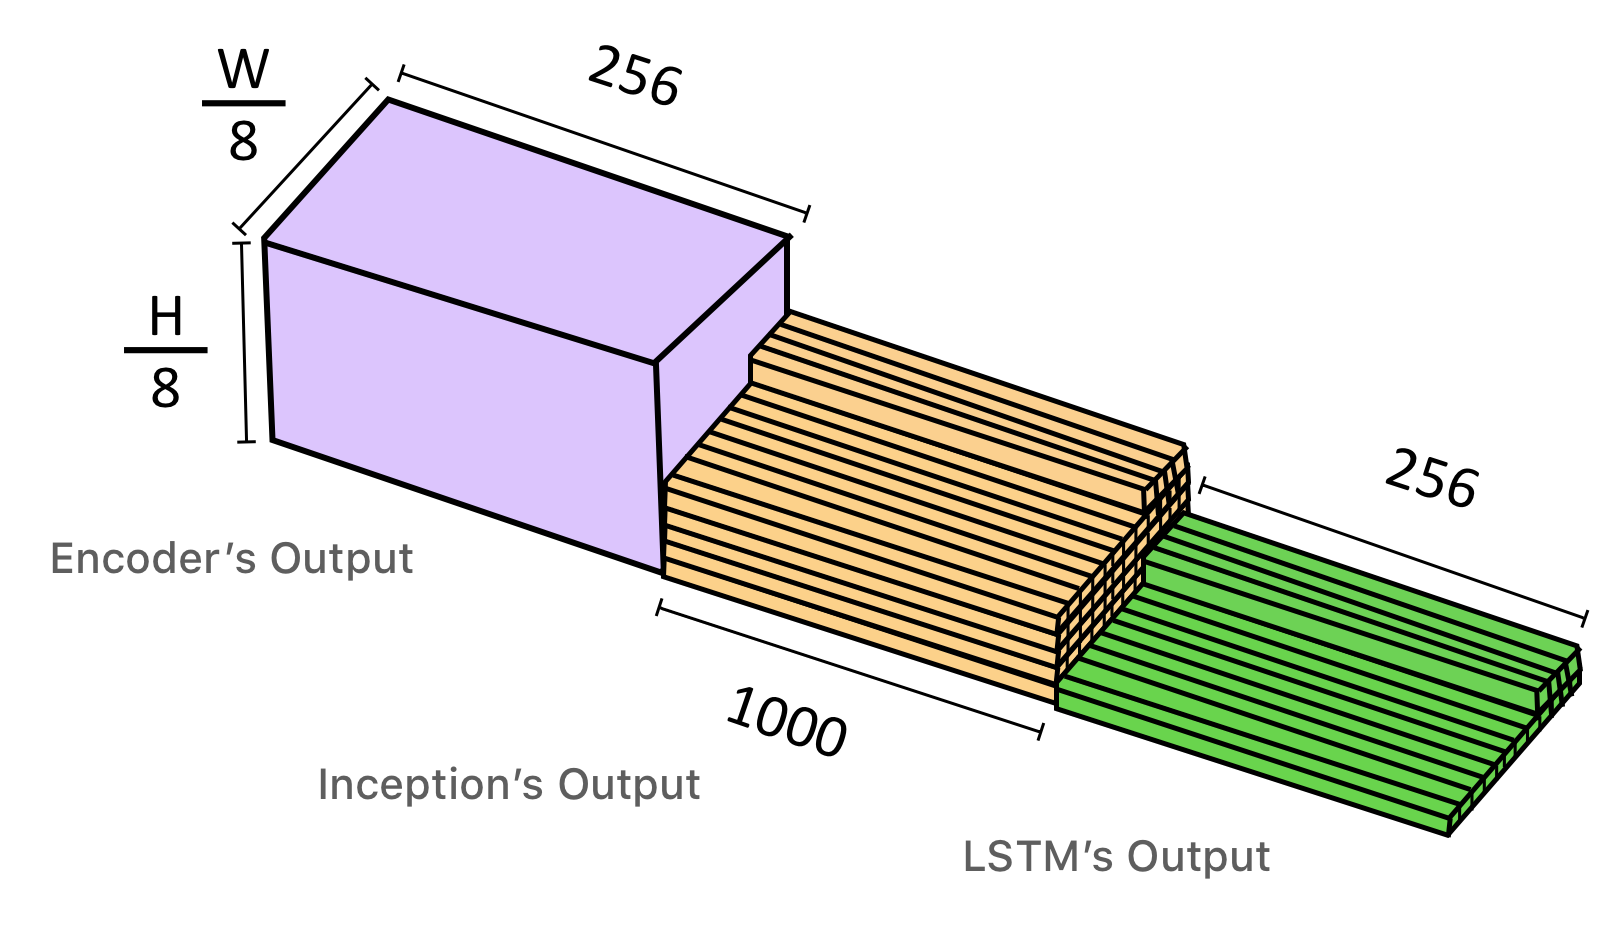
\includegraphics[width=0.5\textwidth]{fusion-layer.png}
  \caption{Fusion Layer - the outputs of the Inception network and the LSTM are replicated and stacked with the CNN encoder's output.}
\end{figure}

\subsection{Colorization Network}
Once the local and global spatial features are fused with temporal features, they are processed by a set of convolutions and up-sampling layers in the CNN decoder. Similar to the CNN encoder and Fusion layer, we apply the CNN decoder to every temporal slice of the input. The decoder takes a $t\times H/8\times W/8\times 1512$ input and results in a final output with dimension of $t\times H\times W\times 2$. The resultant sequence can be considered as the sequence of $a*$ and $b*$ layers for the input sequence of luminance frames, once this result is appropriately merged with the input sequence, we can obtain the final colorized frame sequence.

\subsection{Optimization and Learning}
Optimal model parameters were found by minimizing an objective function defined over predicted outputs and actual results. To quantify the loss, mean squared error between each pixel in $a*$, $b*$ layers of predicted and actual results were used. If we consider a video V, the MSE loss is estimated by,

\begin{equation}
\small
C(X,\Theta ) = \frac{1}{2nHW}\sum_{t=0}^{n}\sum_{k\in {a,b}}\sum_{i=1}^{H}\sum_{j=1}^{W} (X\textsuperscript{k}_{t_{i,j}} - \hat{X}\textsuperscript{k}_{t_{i,j}}) ^ 2
\end{equation}

Here $\theta$ represents all model parameters and $X\textsuperscript{k}_{t_{i,j}}$ represents the $(i,j)$ pixel in $t\textsuperscript{th}$ time frame's $k$ layer. This objective function can be extended to batch level by taking the average 

\begin{equation}
C(X,\beta) = \frac{1}{\left | \beta  \right |}\sum_{X\in {\beta}} C(X,\Theta)
\end{equation}
To optimize the above mentioned objective function, we used Adam optimizer. \cite{DBLP:journals/corr/KingmaB14}

\subsection{Training}
To train the network, approximately 50000 videos from the FCVID \cite{FCVID} video dataset were used, and 10\% of that was treated as validation data. Training was performed on an AWS EC2 instance with 32 virtual CPUs and with four NVIDIA Tesla P100 GPUs giving a total of 64 GB memory. 
Since available computational power was limited, for the moment the model was trained only for videos with five time steps. The used batch size is 20 videos, resulting in around 2150 iterations per epoch. Under the limited resources available, the model was trained for 100 epochs and total training time was close to 50 hours. 

\section{Experiments}
We compare Flowchroma’s video colorization performance by taking the Deep Koalarization framework proposed by Baldassarre et al. as our baseline model. There are mainly two reasons for taking it as our baseline model rather than another image colorization framework or a state-of-the-art technique.
\begin{enumerate}
\item Both FlowChroma and Deep Koalarization use the same transfer learning application of obtaining global features of an image or a video frame from a pre-trained object classifier and fusing them in the fusion layer, similar to Iizuka et al. 
\item The main purpose of our research is emphasizing the use of sequence models in preserving temporal coherence between frames and scene changes rather than extremely realistic colorizations; to achieve that, comparison of our framework with a good enough image colorization framework is sufficient.
\end{enumerate}

To evaluate the performance of FlowChroma against our baseline model, we randomly selected 1000 videos from the FCVID dataset, belonging to various categories depicting a wide range of scenarios, derived their grayscale variants and colorized them with the two models.

In order to provide a fair comparison of the two model’s colorization performance, we used Inception-ResNet-v2, pre-trained object classifier as the global feature extractor for both FlowChroma and the baseline model. We also trained both models for approximately 100 epochs on a part of the same dataset FCVID, keeping 10\% of that as the cross-validation set. Subsequently, a qualitative assessment of the colorizations was performed. 

Our model only takes a sequence of 5 frames as an input at once, but when running inference we need to colorize videos with hundreds of frames. Thus, we use a sliding window approach during inference. In contrast to that, our baseline model only takes a single frame as input at a time, thereby coloring each frame in a video independently.

We first confirm that our model performs well in colorization, and verify that although we use a recurrent architecture, it still converges. Next, we show that we can achieve temporal and contextual coherence through video frames with LSTMs. Finally, we discuss the weaknesses of the proposed architecture and discuss possible solutions.

\section{Results}
In general, we observed that our model produces appropriate colorization results, assigning realistic colors to objects within each scenario. Furthermore, the system successfully maintains color information between frames, keeping a natural flow and a high spatio-temporal coherence at both global and local levels for videos with common objects and environments in the training dataset. We also observed that for objects that are rare or non-existent in the training dataset, our model added bluish flickering patches that followed the movement of the object.

In terms of raw colorization, our model generalizes commonly encountered scenes and objects and assigns them appropriate colors during inference. Figure 3 depicts a scene with a large field in the foreground and a building in the background. The left and right images correspond to the ground truth video frame and output by our model, respectively. Here, our framework discerns that the foreground contains a grassy area, thereby assigning it a lush green color. The ground truth indeed contains a grass field, but it is brown in color, probably due to seasonal effects. This type of colorizations is observed throughout the results and stand to reason that the system generalizes the scenes in the training dataset.

\begin{figure}[!h]
  \centering
  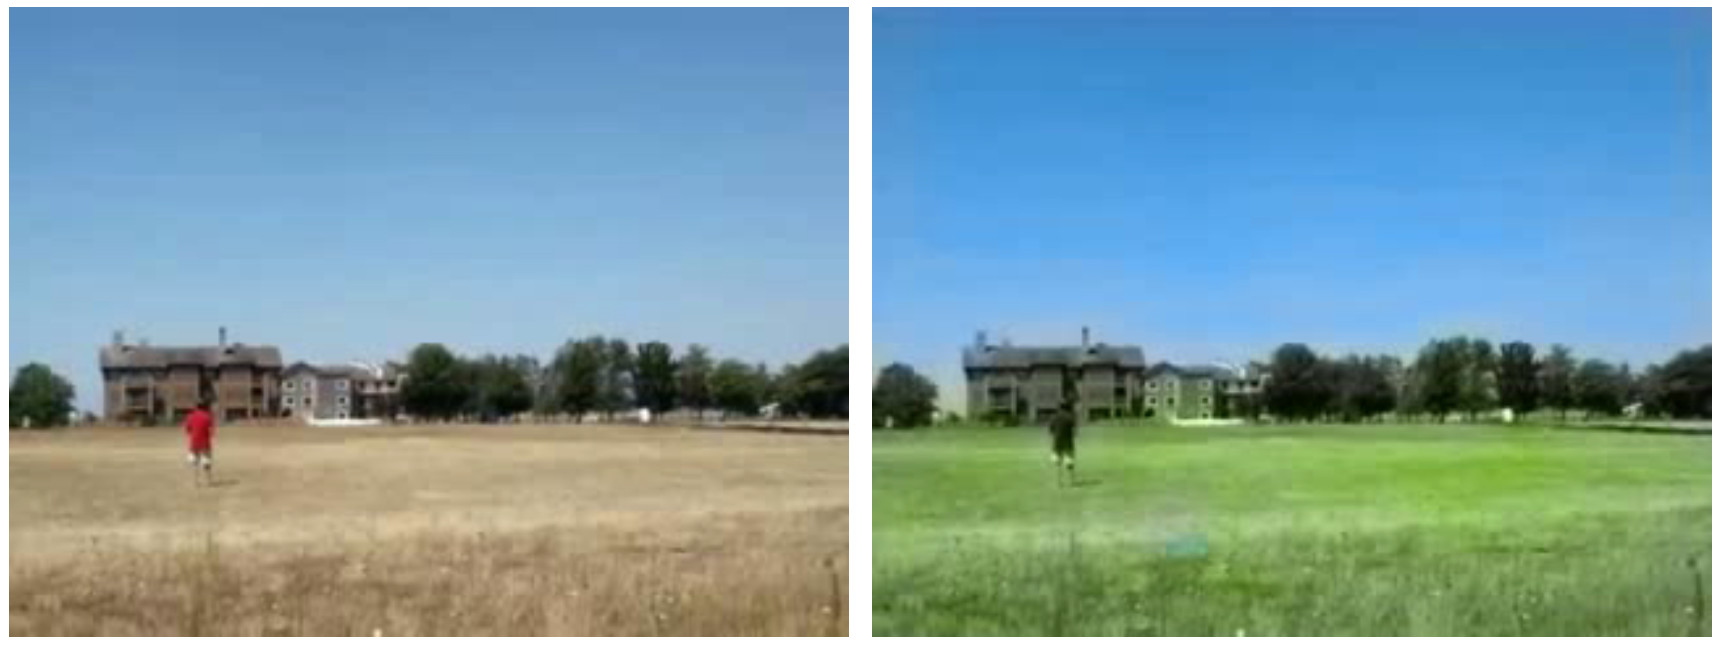
\includegraphics[width=0.5\textwidth]{original-fc-grass-building.jpg}
  \caption{FlowChroma generalizes commonly encountered scenes and objects and assigns them appropriate colors during inference. Here, our framework discerns that the foreground contains a grassy area and assigns it a green color (right), whereas the ground truth is brown (left).}
\end{figure}

\begin{figure}[!h]
  \centering
  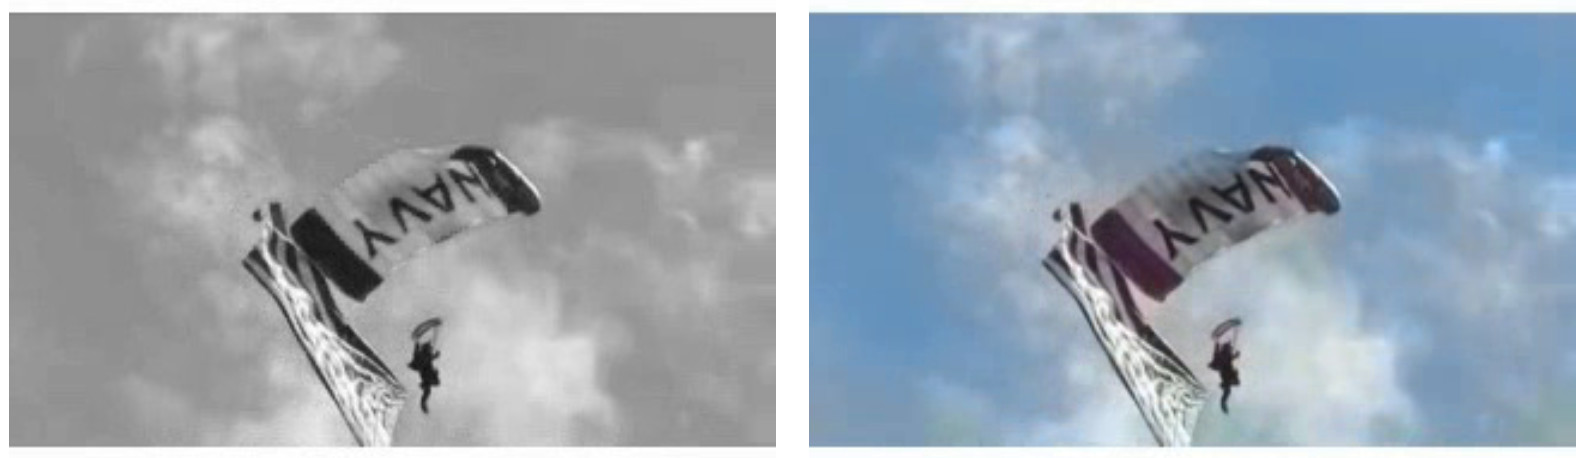
\includegraphics[width=0.5\textwidth]{bw-fc-parachute.jpg}
  \label{}{\footnotesize Fig. 4(a)}
\end{figure}

\begin{figure}[!h]
  \centering
  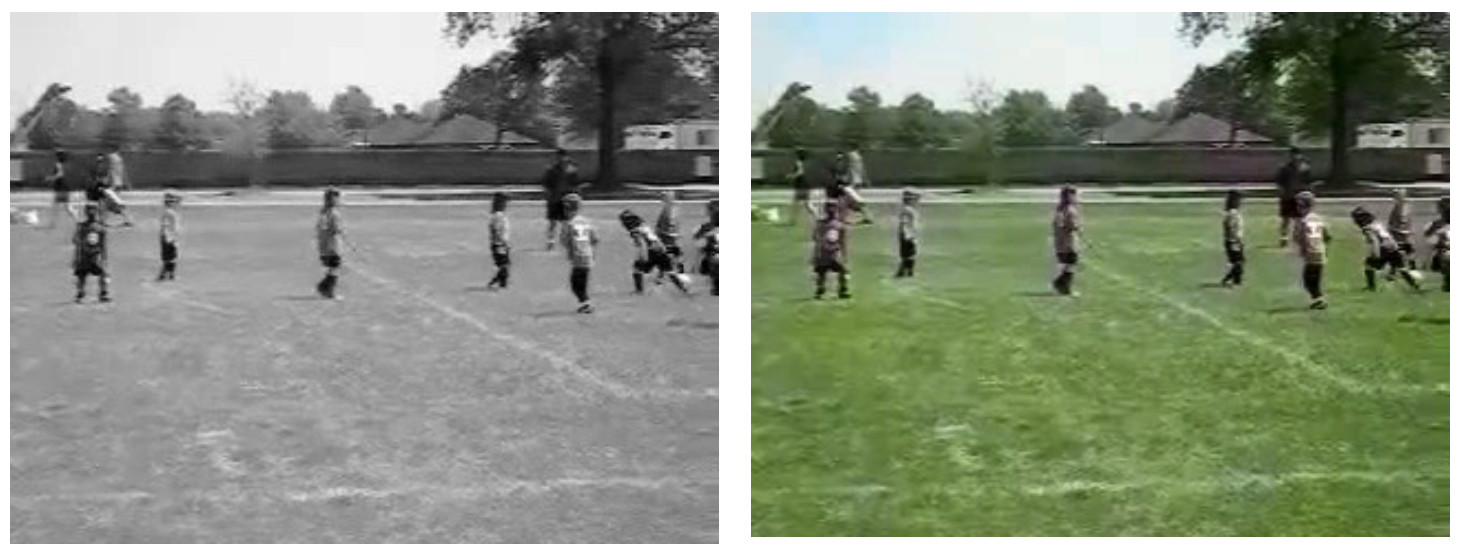
\includegraphics[width=0.5\textwidth]{bw-fc-fifa.jpg}
  \label{}{\footnotesize Fig. 4(b)}
\end{figure}

\begin{figure}[!h]
  \centering
  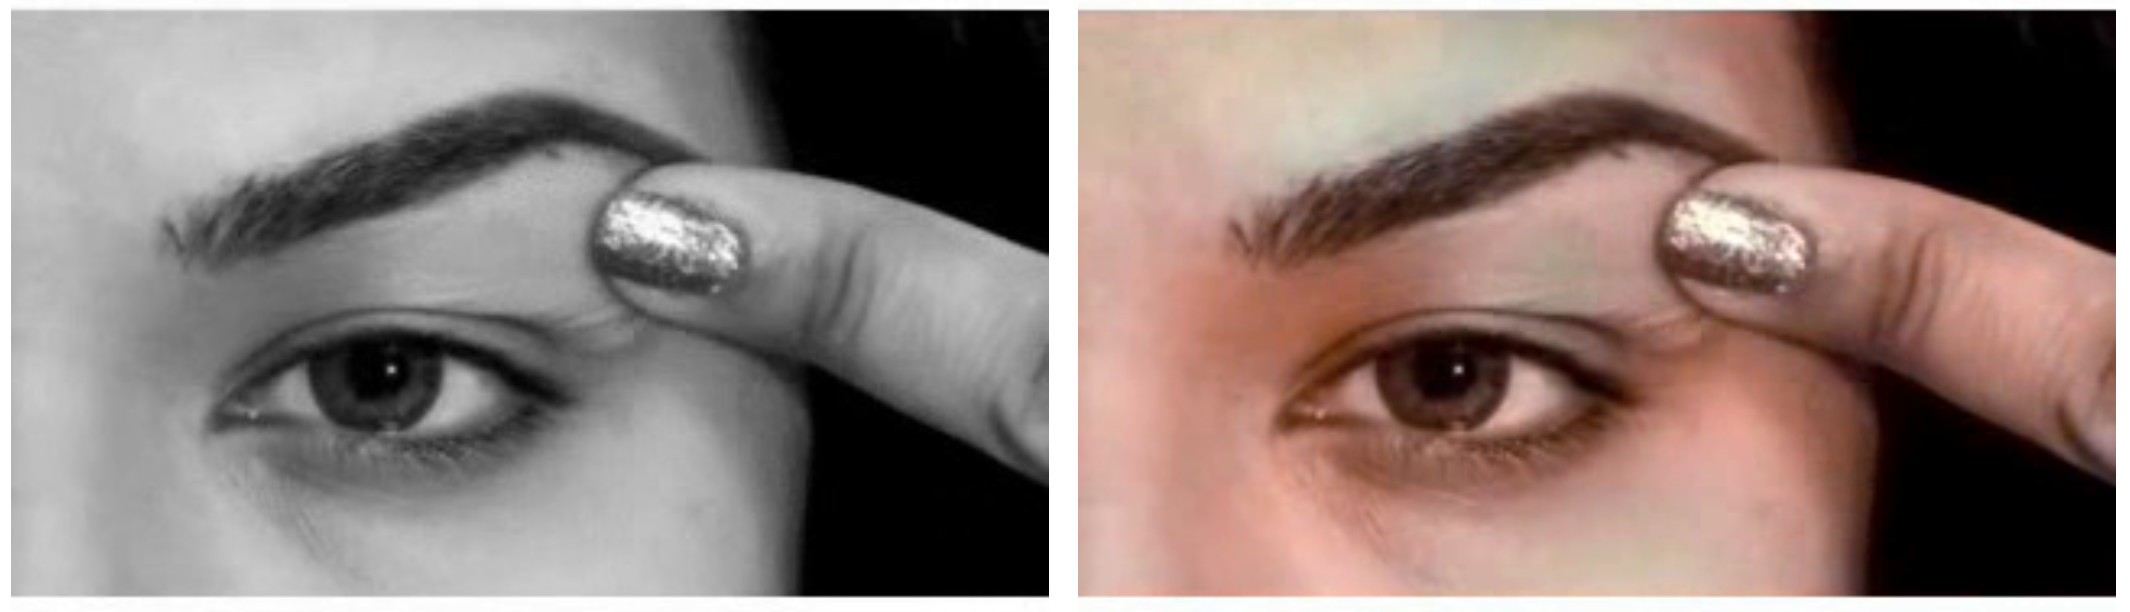
\includegraphics[width=0.5\textwidth]{bw-fc-lady-face.jpg}
  \label{}{\footnotesize Fig. 4(c)}
  \caption{FlowChroma generates a considerable variation of colors in each scene throughout the colorization results, as demonstrated by this set of figures. In first row, Note how the parachute and the flag are colored in red hues while the sky is in blue. In third row, the eye color and skin tones over different regions in the face make the frame appear more realistic.}
\end{figure}

The novelty in our model lies in the use of LSTMs to maintain contextual frame information across time, and we observe its effects on colorization at two scales;  locally and globally. At a global level, Flowchroma maintains the overall color composition of a scene throughout the video better than the baseline image colorization model. At a local level, the baseline model sometimes mistakenly colorizes small regions of a frame with inappropriate colors, but Flowchroma avoids such mistakes.

An example of this is shown in Figure 5(a), which depicts a herd of elephants strolling about. FlowChroma keeps the dry tone of the environment across the video while the baseline model shows colors changing between green and off-brown. Similarly, in 5(b), FlowChroma again maintains the grass field in green while the baseline flickers from brown to green. In 5(c), note how the baseline system bleeds color from the smartphone’s clock into the background while our model does a better job of keeping the background uniform. 

\begin{figure*}[!h]
	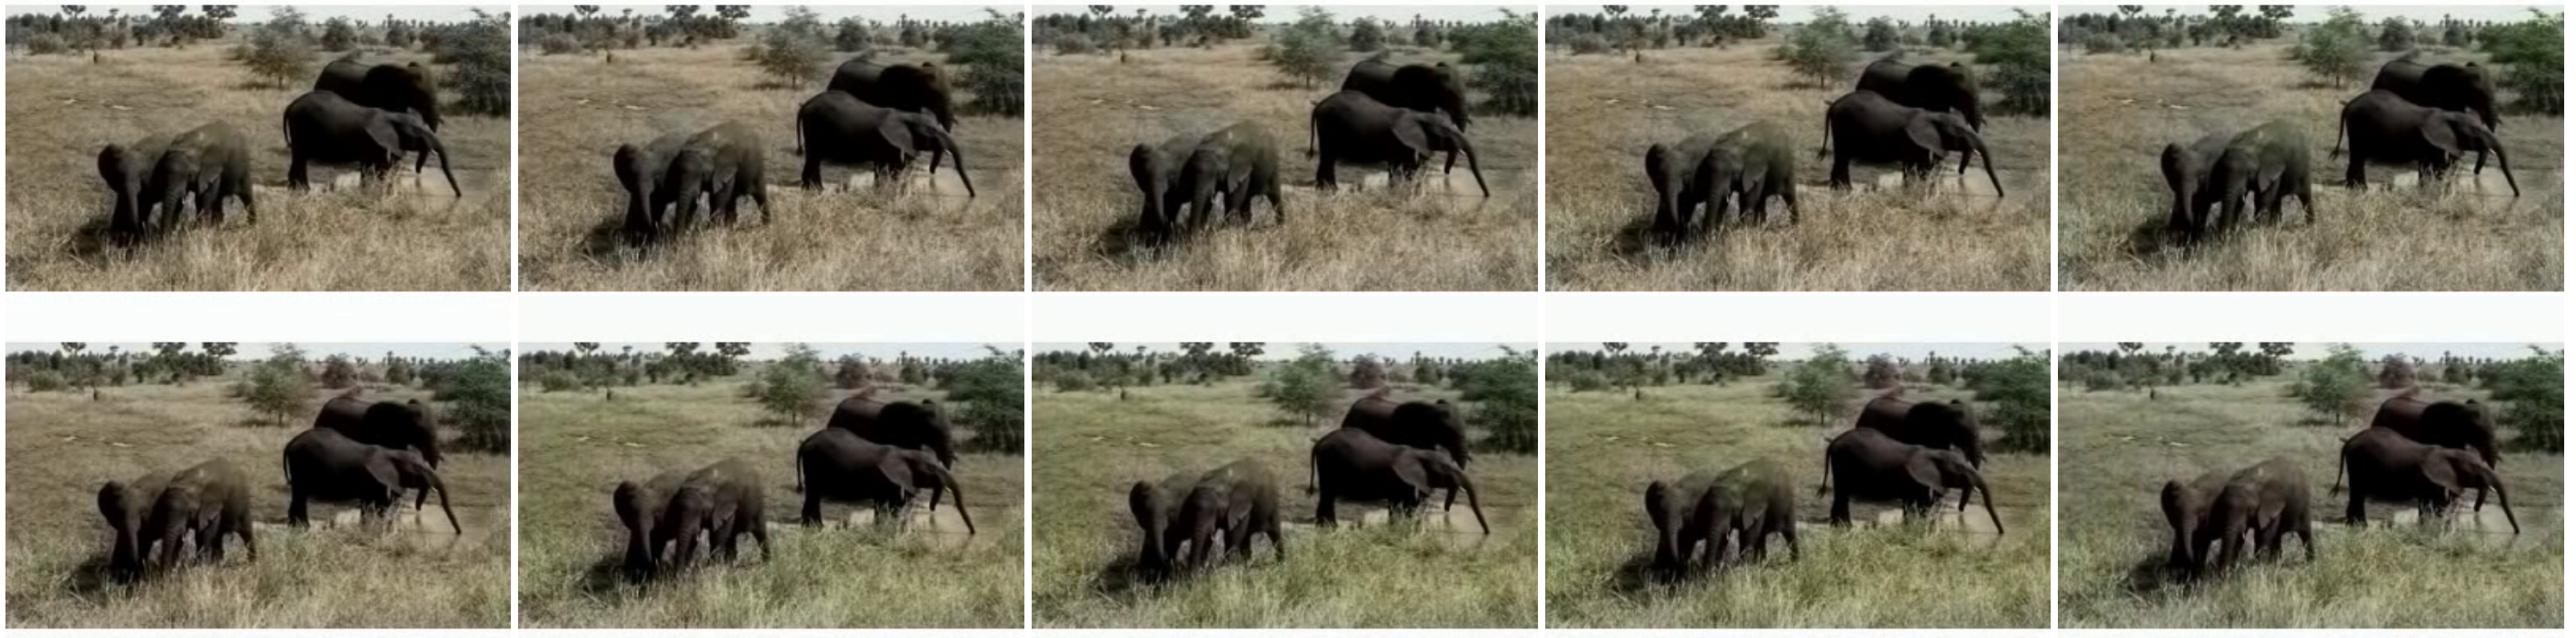
\includegraphics[width=\textwidth]{fc-dk-elephants.jpg}
    \centering
    \label{}{\footnotesize Fig. 5(a)}
\end{figure*}
\begin{figure*}[!h]
	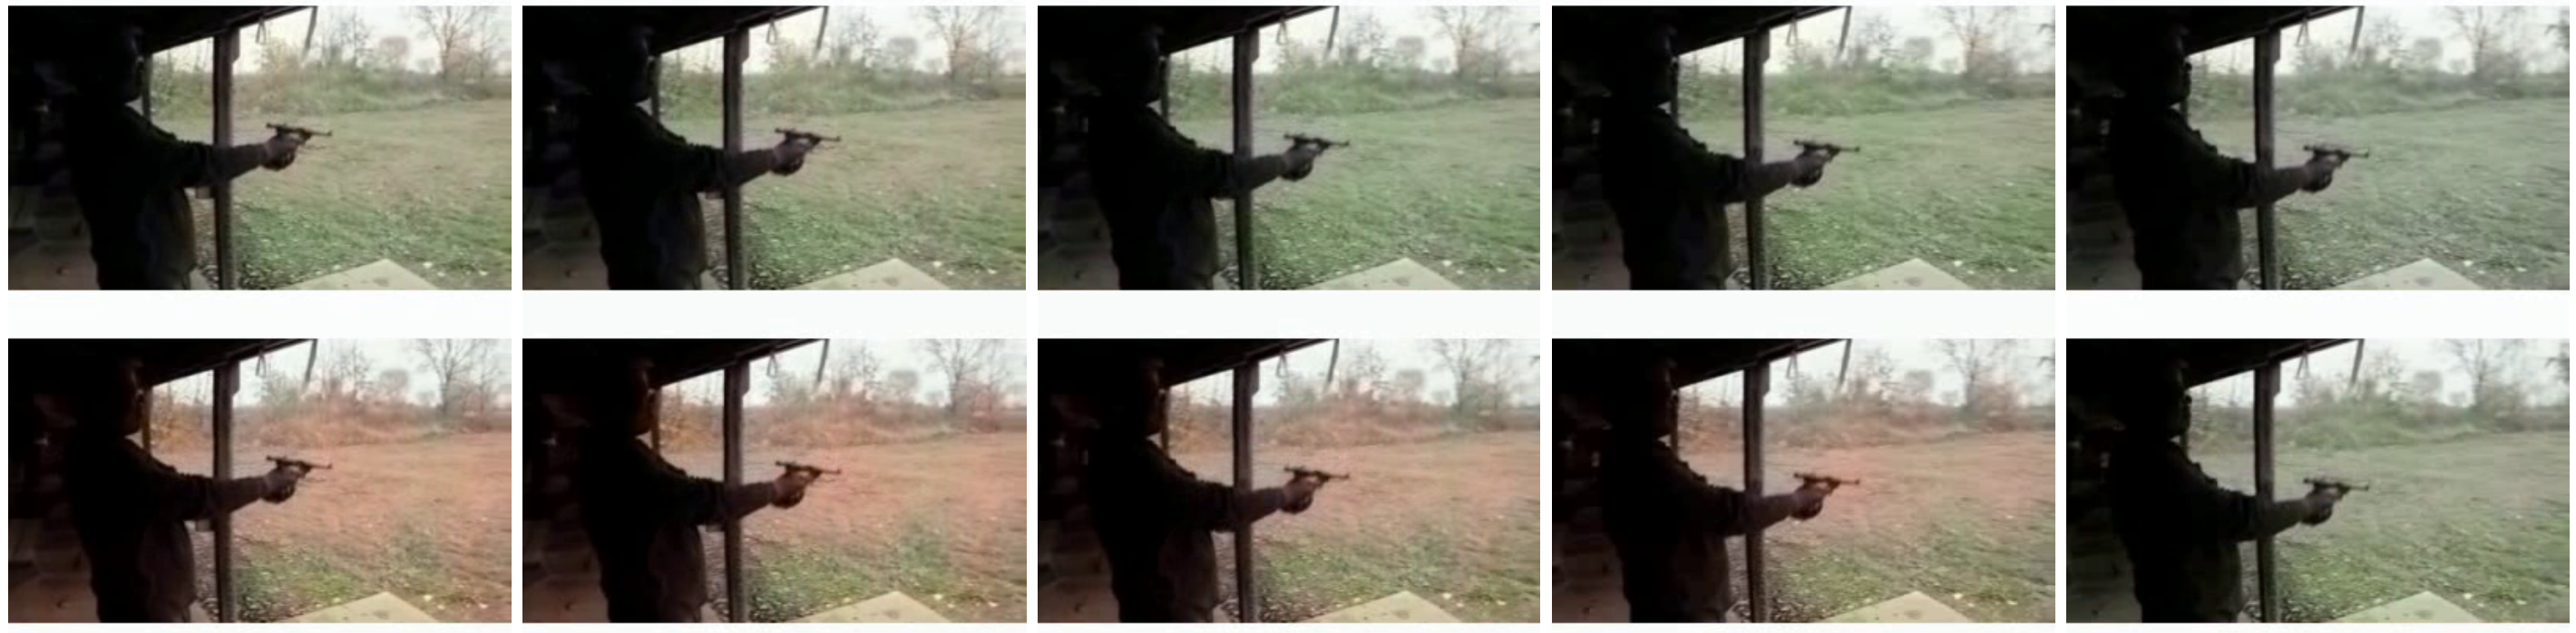
\includegraphics[width=\textwidth]{fc-dk-shooting.png}
	\centering    
    \label{}{\footnotesize Fig. 5(b)}
\end{figure*}
\begin{figure*}[!h]
	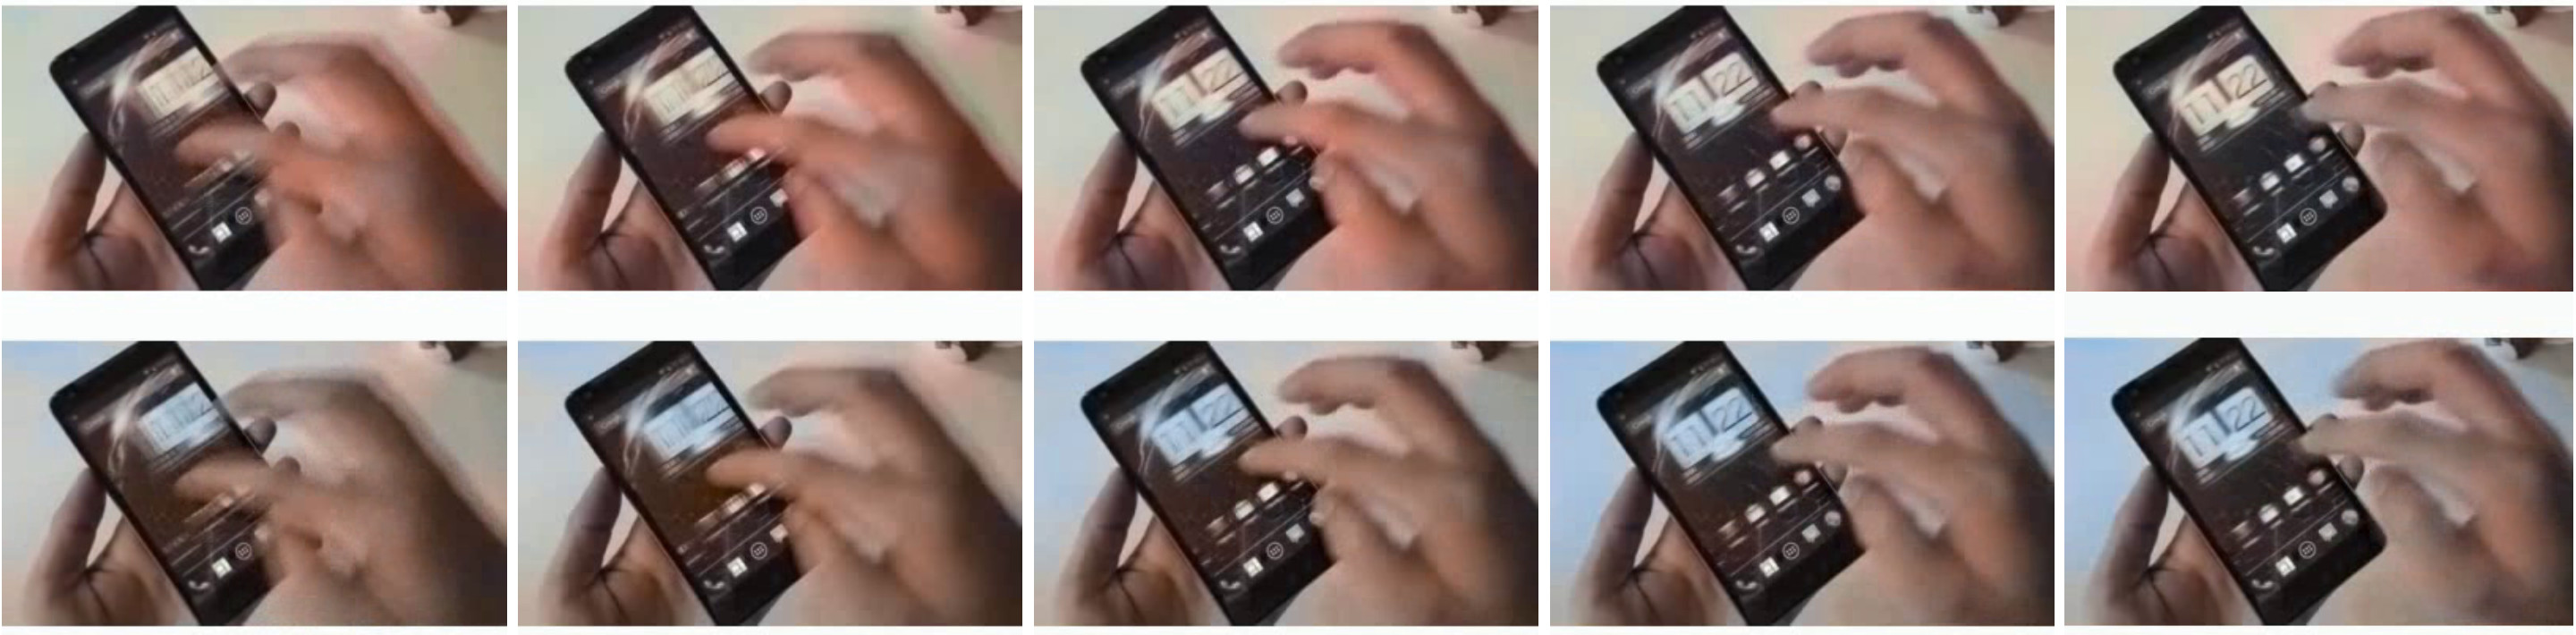
\includegraphics[width=\textwidth]{fc-dk-mobile-phone.jpg}
	\centering
    \label{center}{\footnotesize Fig. 5(c)}
    \caption{In each of the figures 5(a), (b) and (c), the top and bottom rows show the video frame sequences colored by FlowChroma and the baseline model respectively. These show the superior global color palette maintenance throughout the scene by the LSTM.}
\end{figure*}

\begin{figure*}[!h]

\includegraphics[width=\textwidth]{fc-dk-baby-tub.png}
\centering
\label{}{\footnotesize Fig. 6(a)}
\vspace{5.00mm}
\end{figure*}

\begin{figure*}[!h]

\includegraphics[width=\textwidth]{fc-dk-playing.png}
\centering
\label{}{\footnotesize Fig. 6(b)}
\caption{The two figures 6(a) and 6(b) show video frame sequences of FlowChroma (top row) and the baseline model (bottom) in which the local color uniformity is better maintained by FlowChroma. Note how the baseline model flickers with blue color patches.}
\end{figure*}

At a local scale, the LSTM affects how FlowChroma decides colors should be assigned even when it cannot fully identify the progression of a previously detected region. In Figure 6(a), the background contains a wall that is uniformly colored throughout the frames by FlowChroma, while having blue patches in the baseline model’s output. This is an example of the downsides of considering each frame as a separate colorization task, as done by image colorization models. Figure 6(b) contains an off-white board that is consistently colored by FlowChroma, whereas the baseline model again adds blue color patches.

In Figure 5, the baseline model correctly identifies the background as vegetation, and only fails to maintain consistent colors. In Figure 6, bluish spots are introduced by the baseline model probably due to erroneously identifying those regions as sky or water in some frames. But FlowChroma avoids such mistakes as once it identifies the vegetation and assigns a color, it tries to maintain that color.

We can divide the factors affecting the consistency of colorization as temporal and non-temporal. Non-temporal factors include extreme pixel values such as black (0) or white (255), and the prevalence of a context in the training dataset. These factors affect both image colorization extensions to video colorization as well as FlowChroma. If the pixel values are extreme, such as in the case of snow or asphalt roads, both the baseline model and FlowChroma tend to leave them as they are without assigning new colors. Furthermore, when colorizing commonly encountered contexts such as blue sky or green pastures, both the baseline and our model again keep the colors consistent with minimal flickering. The reason is that Inception-ResNet-v2 is pre-trained on the ImageNet dataset, which contains  images of commonly encountered context. This factor is mainly applicable to models that use global context identification for colorization; e.g. Iizuka et al., Baldassare et al.

Temporal factors mainly relate to the movement of objects in a scenario, where the action frequency confuses the system's perception of the trajectory of the scene. This is applicable only to FlowChroma. When the movements in a video are smooth, the system identifies the objects and applies appropriate, temporally coherent coloring. When the movement in the scenario speeds up, the perceived flow of movement breaks and thus the colorization quality degrades.

Lastly, we observe when FlowChroma’s colorization becomes inconsistent and propose possible solutions. When there is a high object frequency in a scene, the aptness of the colorization gets reduced. An example would be a surface with a complex pattern. A potential solution would be to train the system on more videos with high object frequency. The action frequency also adversely affects the system performance. Normalizing the action speed is one possible solution. This could be done by increasing the number of frames containing the movement by predicting intermediate frames, as recently demonstrated by Nvidia \cite{DBLP:journals/corr/abs-1712-00080}, and then slowing down the video to achieve the desired speed. Another potential solution is to train the system with more time steps. 

Furthermore, the introduction of new objects into a scene changes its context and the model suddenly gets confused, introducing momentary flickering before stabilizing again. Training the model further may alleviate this problem. Finally, if an object is uncommon or non-existent in the training dataset, the system shows poor performance in identifying the object boundaries. This could be fixed by expanding the dataset to cover a broader set of objects.


When the movements in a video are smooth, most of the time the system identifies the objects and applies appropriate, temporally coherent coloring. When the movement in the scenario speeds up, the flow of movement breaks and thus the colorization quality degrades fast, especially in terms of segmentation and appropriate coloring.

\section{Conclusions}

Contemporary image colorization techniques are not directly applicable to video colorization as they treat each video frame as a separate colorization task without maintaining temporal coherence between frames. We propose FlowChroma, a novel colorization framework with a recurrent neural network - LSTM - added to maintain temporal and contextual information between frames. We show that the LSTM maintains the image colorization quality of current methods intact while also successfully minimizing flickering between frames. It maintains the overall color palette of a scenario across subsequent frames at a global level, while coloring identified objects within a scene consistently at a local level. 

The use of LSTM also has some drawbacks; firstly, color consistency is degraded when a new object suddenly comes into the frame. Secondly, fast movements in a scene confuses the LSTM's understanding of the movement, which causes colors to bleed out from object edges and introduces blobs of flickering. One potential solution would be to normalize the speed of movements. Furthermore, we observed that the main causes of flickering in FlowChroma are high action and object frequency, and the sudden introduction of new objects into a scenario. 

We achieve the goal of maintaining temporal and contextual coherence in video colorization with LSTMs and as future work, we hope to develop a video colorization benchmark with a standardized dataset.


%-------------------------------------------------------------------------



{\small
\bibliographystyle{ieee}
\bibliography{egbib}
}


\end{document}
